\section{Proposed Method}
\label{sec:method}
\begin{figure*}
    \begin{center}
        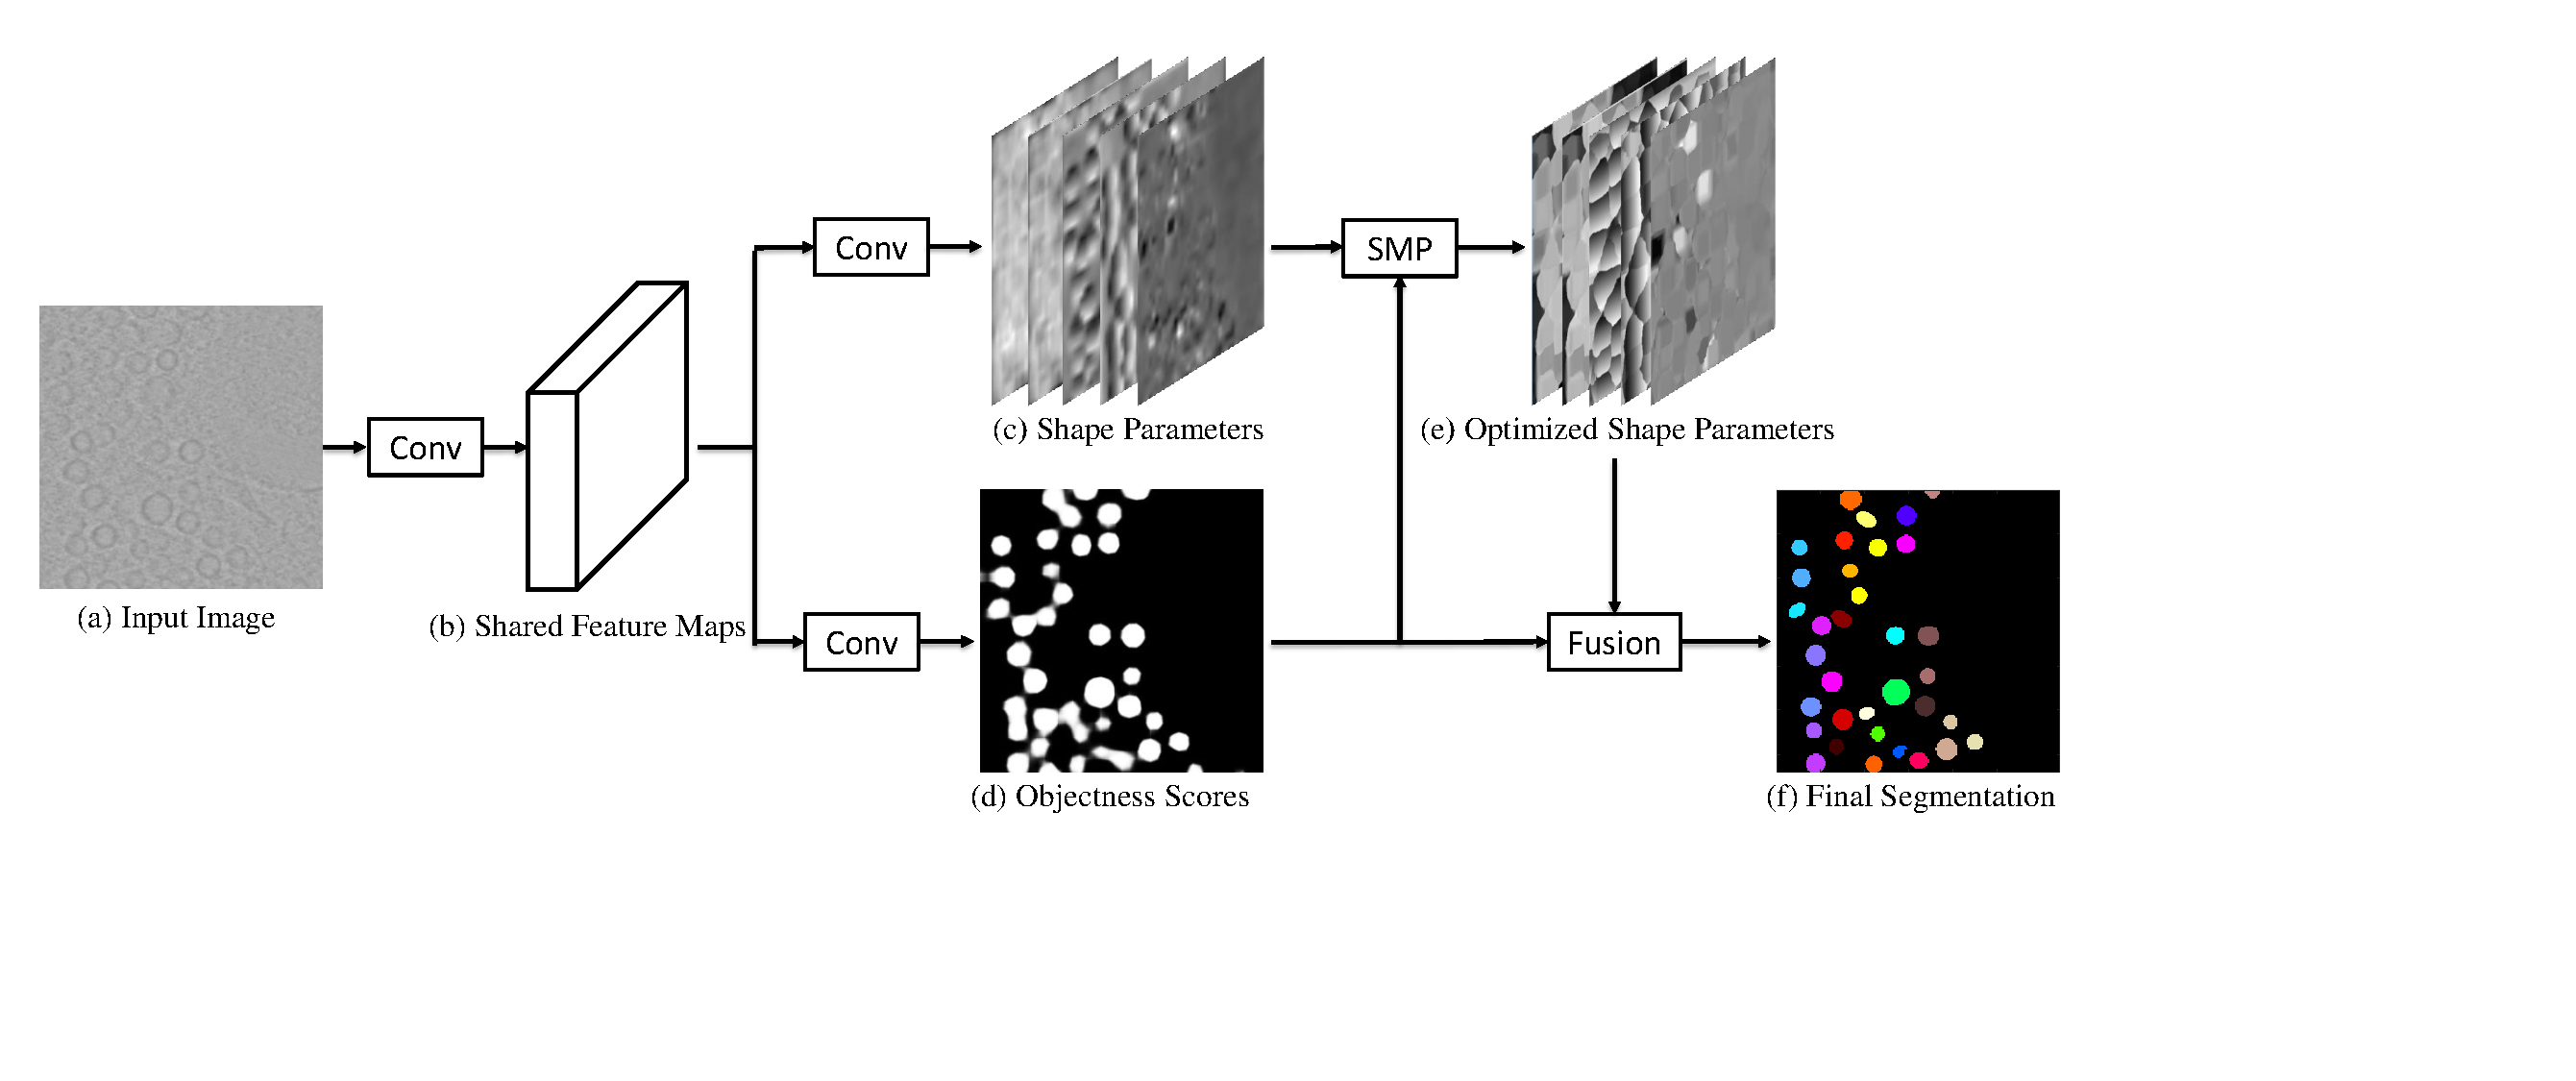
\includegraphics[width=6.7in]{figures/FigDSAN.pdf}
    \end{center}
    \caption{Overview of our proposed DSAN. Given an image (a), a multi-task network simultaneously predicts an objectness score map (d) and several shape parameter maps (c) based on the shared feature maps (b).
    Then a split max pooling (SMP) pools the shape parameters (c) using objectness score (d), which gives the optimized shape parameters (e).
    Finally, the segmentation mask (f) is obtained by fusing (d) and (e) (Piecewise fusion).}
    \label{FigDSAN}
\end{figure*}

A complete pipeline of Deep Shape-Aware Network (DSAN) is illustrated in Figure~\ref{FigDSAN}.
The framework is trained end-to-end and consists of three key components:
1) a deep multi-task network based on FCN (Sec.~\ref{sec:multi-task-fcn}),
2) proposed split max pooling (Sec.~\ref{sec:split-max-pooling}) and
3) piecewise fusion strategy to generate the final segmentation mask (Sec.~\ref{sec:fusion}).

\subsection{Multi-task FCN}
\label{sec:multi-task-fcn}

The architecture of our multi-task learning network is shown in Figure~\ref{FigDSAN}.
It simultaneously predicts an objectness map $P$ and several auxiliary maps $\{T_k\}_{k=1,\ldots,K}$ as complementary information.
The feature extracting part is shared and based on DeepLab~\cite{Chen2014a}, which introduce the dilated convolution layers into FCN for lager reception field.
%Instead of powerful ResNet~\cite{Zhao2016} and recent DenseNet~\cite{Huang2016} to extract feature, we choose FCN to demonstrate the superiority of our shape-aware framework in resolving touching problem compared to existing FCN based methods for biomedical segmentation.
Then, the feature maps extracted by last shared convolution layer are fed into two individual branches.
%In each branch, successive two convolution layers are applied to the input feature maps with stride $1$ and kernel size $3\times 3$ and $1\times 1$ respectively.
%Then the outputs of each branch are upsampled to match the original image using bilinear interpolation.
In each branch, two successive convolution layers are applied to the shared feature maps and an upsample layer restore the predictions to the original image size.
During training, the parameters of shared layers are jointly optimized, while the parameters of two branches are updated independently.

Instead of directly predicting contour probabilities in \cite{Chen2017,Chen2016,Bertasius2016}, we choose the parameterized expression of objects shape as complementary information, which emphasizes more on the overall shape of objects to be segmented.
For example in vesicle segmentation, since the shape of most vesicle objects are approximately ellipse, we choose the ellipse as the prior shape knowledge and express them with the parameters $\{\theta, \mu_c, \nu_c, a, b\}$.
$\theta$ is the rotated angle of major axis from $x-$axis.
$(\mu_c, \nu_c)$ are the coordinates of the ellipse center.
And $a$, $b$ are respectively the lengths of major and minor axes.
With these definitions, the auxiliary maps has $5$ channels and each $T_k$ predicts one of the five parameters.
Especially for pixel $i$, the predicted shape parameters $\mathbf{t}_i= \{T_{1,i},\ldots,T_{5,i}\}$ formulate the shape of the nearest object to pixel $i$.
For better regression, the shape parameters are further normalized by image width $W$ and height $H$ so that they fall in $[0,1]$:
\begin{eqnarray}\label{EqPara}
\begin{aligned}
\mathbf{t}_{i} = \{\theta,\frac{\mu-\mu_c}{W},\frac{\nu-\nu_c}{H},\frac{a}{H},\frac{b}{H}\}
\end{aligned}
\end{eqnarray}
where $(\mu, \nu)$ are spatial coordinates of pixel $i$.

Finally inputting an image, the objective function of our multi-task FCN is defined by:
\begin{eqnarray}\label{EqLoss}
\begin{aligned}
L(P,\{T_k\}) =& \frac{1}{N}(\sum_{i}L_{cls}(P_i,P^*_{i})+\\
&\lambda\sum_{i}\sum_{k}P^*_{i}L_{reg}(T_{k,i},T^*_{k,i}))\\
\end{aligned}
\end{eqnarray}
where $N$ is the total number of pixels.
$P^*_i$ and $T^*_{k,i}$ are the ground truth of objectness score and $k$-th shape parameter at pixel i.
The classification loss $L_{cls}$ is the soft-max loss and regression loss $L_{reg}$ is defined by
\begin{eqnarray}
\label{EqSmoothL1}
\begin{aligned}
L_{reg}(t_1,t_2) =\left\{\begin{array}{cc}
0.5(t_1-t_2)^2&if~|t_1-t_2|<1\\
|t_1-t_2|-0.5&else\\
\end{array}\right.
\end{aligned}
\end{eqnarray}
which is the smoothed $L_1$ loss for robust regression in \cite{Ren2015}.

Especially in Eq.~\ref{EqLoss}, we only consider the regression loss with positive $P^*_i$, because most $T_{k,i}$ with negative $P^*_i$ will be replaced in next section by proposed split max pooling.
And $\lambda$ is a balancing weight between $L_{cls}$ and $L_{reg}$.

\subsection{Split Max Pooling}
\label{sec:split-max-pooling}
\begin{figure}
    \begin{center}
        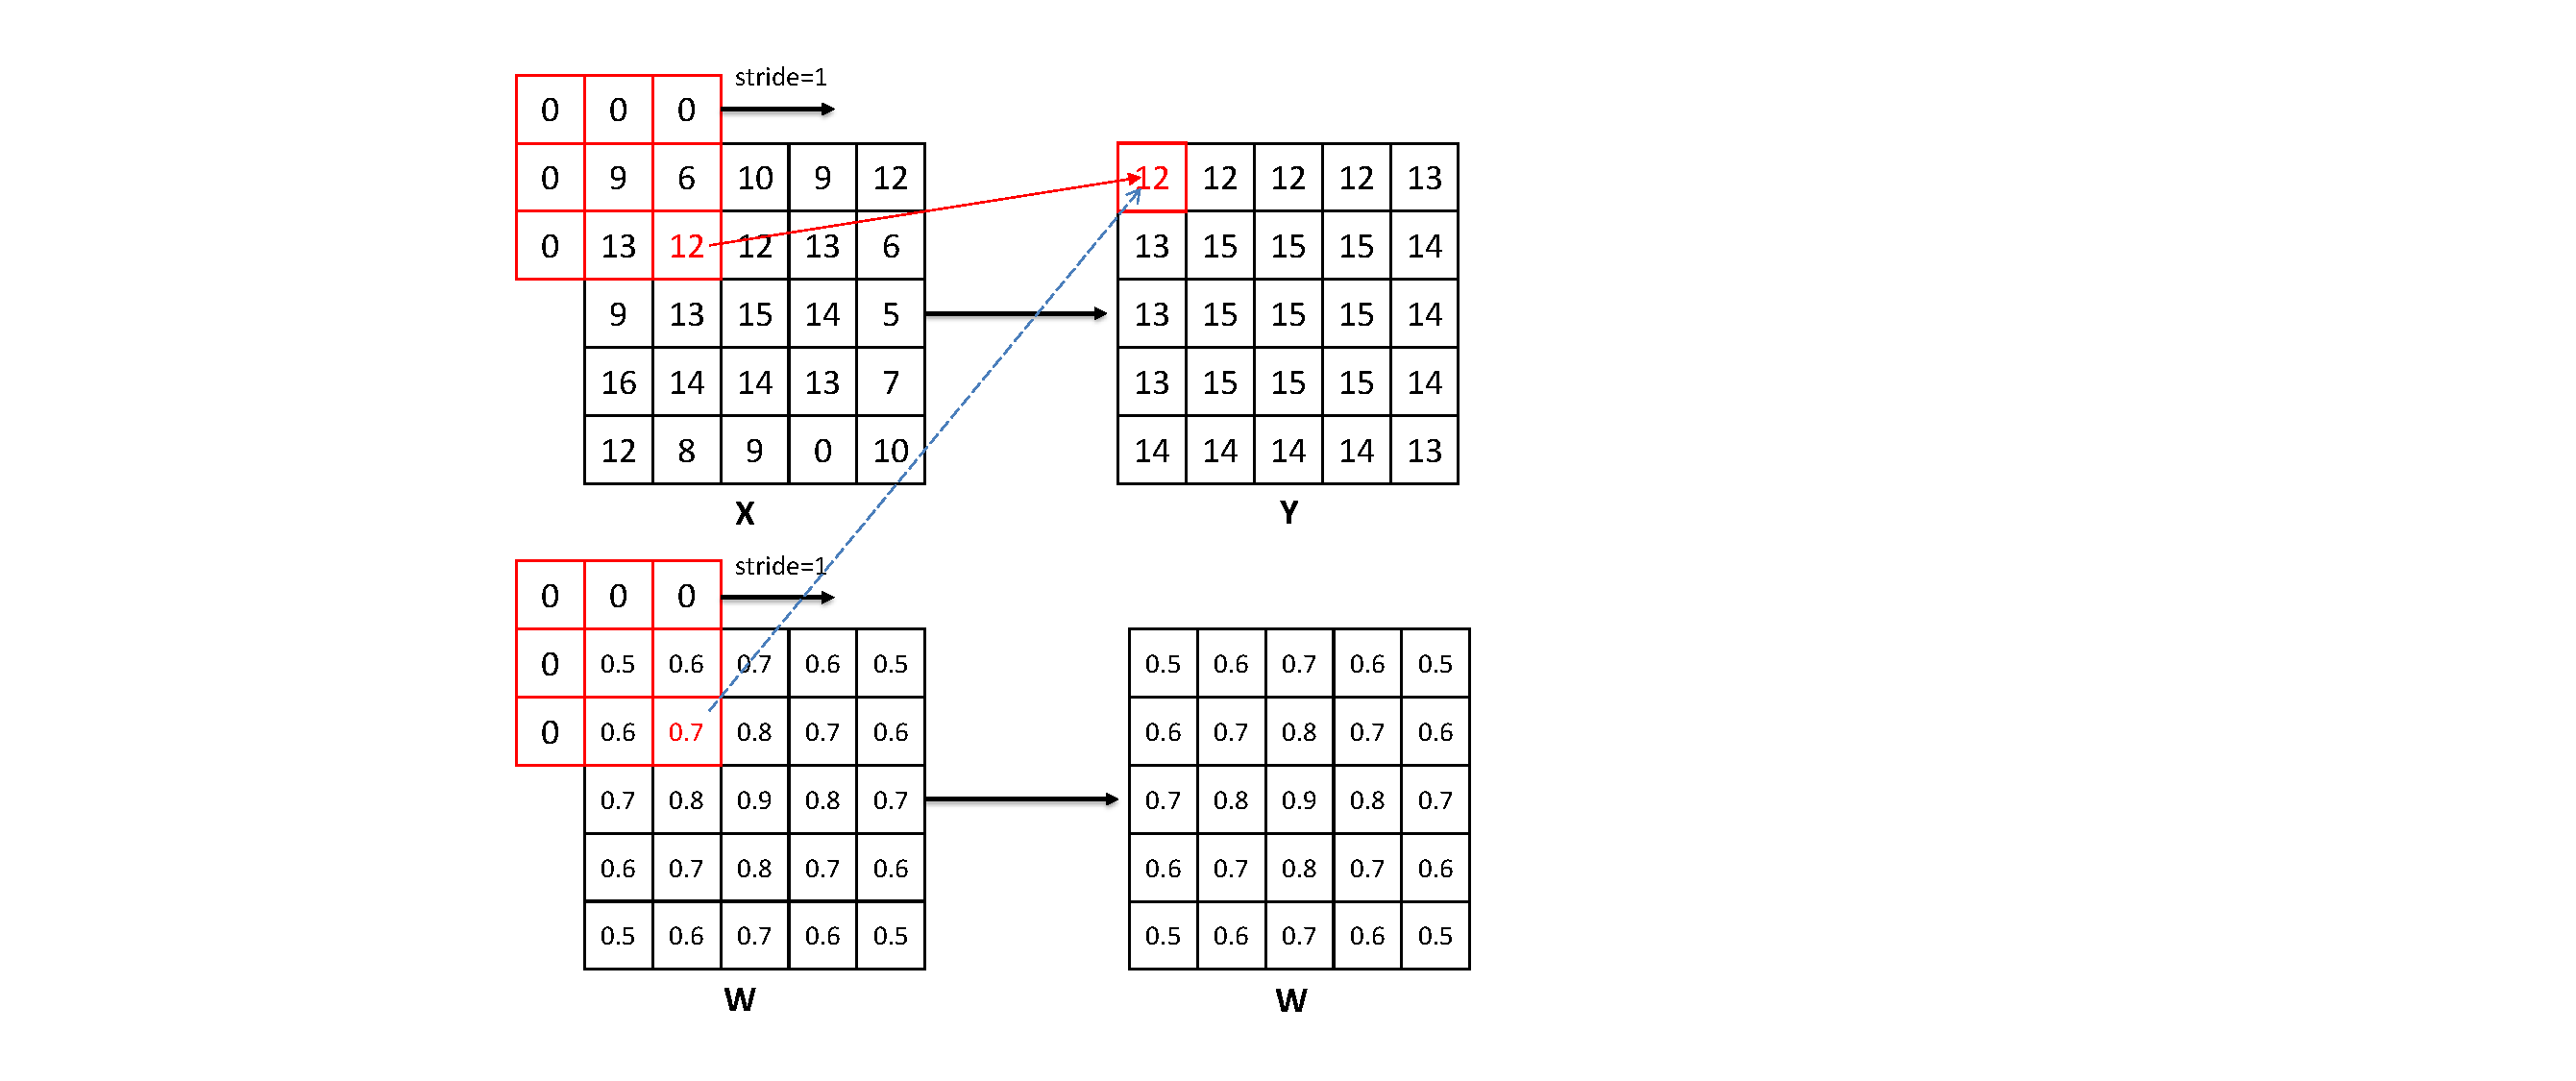
\includegraphics[width=3.2in]{figures/FigSMP.pdf}
   %\includegraphics[width=0.8\linewidth]{egfigure.eps}
    \end{center}
    \caption{An example of split max pooling.
        Two windows of the same size synchronously slide on $X$ and $W$.
        In the top window, only $x$ with maximal score $\omega$ in the bottom window will be propagated to the next layer.
        And $W$ will be unchanged and reused for next split max pooling during forward propagation.}
    \label{FigSMP}
\end{figure}

Obtained from two individual branches of multi-task FCN, the predicted shape parameters in auxiliary maps are not accurate enough to optimize the objects shape predicted by objectness map as shown in Table~\ref{tab:var}.
This is caused by different perception field needed to explore an object at different position.
Usually, a larger perception field is needed by predicting at boundary region than that in central region, thus the central predictions of an object are more accurate.
To this end, we introduce a novel split max pooling (SMP) to improve the accuracy of auxiliary predictions in boundary region of objects by utilizing the complementary information in objectness scores.
Different from conventional max pooling, our SMP takes two maps as inputs and pools one with the other one, of which the back propagation can further benefit both inputs by their inherent association.

A conventional pooling operation can be expressed as
\begin{eqnarray}\label{pooling}
\begin{aligned}
y_{j} = \sum_{i\in \mathcal{N}_{j}} \omega_{i}x_{i}
\end{aligned}
\end{eqnarray}
where $\mathcal{N}_{j}$ is a neighbor region of pixel $j$ according to the sliding window, and $\omega_{i}$ is the weight of pixel $i$.
For traditional max pooling, $\omega_i \in \{0,1\}$ is a binary indicator for whether $x_i$ is the maximum in the local region.
%There is only one pixel in the neighborhood has $\omega=1$ and all the others have $\omega=0$.
For an average pooling, all pixels in the local window take the identical weight $\omega=\frac{1}{N}$, where $N$ is the total number of pixels in the local region $\mathcal{N}$.
Intuitively, $\omega$ acts like an $``$indictor" determining the pooling strategy of $x$.

Based on this observation, we proposed a split max pooling (SMP) operation, of which the $\omega$ is generated from an independent input, rather than $x$.
Explicitly, our SMP takes two inputs: $X$ and $W$, corresponding to the auxiliary map $T_k$ and objectness map $P$ respectively in our task.
During forward propagation, two windows with same size, denoted by $\mathcal{N}^{x}$ and $\mathcal{N}^{\omega}$, synchronously slide on $X$ and $W$.
%$\mathcal{N}^{x}$ and $\mathcal{N}^{\omega}$ has the same perception field $\mathcal{N}$ on different input maps.
%The $\mathcal{N}^{x}$ is the pooling window, while $\mathcal{N}^{\omega}$ is the decision window.
The elements in $\mathcal{N}^{x}$ will be pooled and propagated to next layer under the pooling strategy determined by $\mathcal{N}^{\omega}$.
%The pooling strategy in $\mathcal{N}^{x}$ will be determined according to the elements in $\mathcal{N}^{\omega}$.
The forward propagation of split max pooling can be expressed by:
\begin{eqnarray}\label{smp}
\begin{aligned}
y_{j} &= \sum_{i\in \mathcal{N}_{j}}x_{i}\hbar(\omega_{i},\mathcal{N}^{\omega}_{j})\\
\hbar(\omega_{i},\mathcal{N}^{\omega}_{j})&=\left\{\begin{array}{cc}
1&if~\omega_{i}\geq max(\mathcal{N}^{\omega}_{j})\\
0&else\\
\end{array}\right.
\end{aligned}
\end{eqnarray}
As $\omega_i$ is the element in $\mathcal{N}^{\omega}_{j}$, only the maximal element of $\mathcal{N}^{\omega}_{j}$ can give a positive output of function $\hbar$.
A simple example of Eq.~\ref{smp} is shown in Figure~\ref{FigSMP}.
And we can forecast that $Y$ will be gradually filled by $x$ with the maximum $\omega$, along with this process iterated.

In our segmentation task, we find that the objectness score $P_i$ in central region of an object are usually the local maximum.
Therefore, our SMP is able to replace the predicted shape parameters $T_{k,i}$ in boundary region with that in central region of an object, which are usually more accurate.
Especially, the pooling stride is fixed to be $1$ to maintain an unchanged resolution of output map, while the pooling size and iteration times of SMP jointly determine the spreading range of a $T_{k,i}$ with maximum $P_i$.

Another contribution of our SMP is that the residual error can be correctly back propagated to its inputs.
This makes it a trainable layer in any network architecture and our DSAN become an end-to-end system.
Defining $L$ as the residual error, the back propagation for $x_{i}$ can be expressed by:
\begin{eqnarray}\label{bpx}
\begin{aligned}
\frac{\partial L}{\partial x_{i}}=\frac{1}{m}\sum\limits_{j\in\mathcal{N}_{i}}\frac{\partial L}{\partial y_{j}}\hbar(\omega_{i},{\mathcal{N}}^{\omega}_{j})\\
\end{aligned}
\end{eqnarray}
where $\mathcal{N}^{\omega}_{j}$ is the neighbor region centered at position $j$ of $W$ and $m$ is the number of elements in $\mathcal{N}_{i}$.
Similar to forward propagation of original max pooling, Eq.~\ref{bpx} converge the gradients $\frac{\partial L}{\partial y_{j}}$ into the $x_{i}$ that has a local maximum $\omega_{i}$.
With most residual error of $T_{k,i}$ converged at the pixels with maximum $P_i$, the predicted shape parameters in central region of objects will be more accurate.

%Specially in Figure \ref{FigSCNN}, the input segmentation map is assumed to not only influence the output but also feeds a subsequent layers, thus also receiving gradient contributions $\frac{\partial L}{\partial s_{i,j}}$ from the next layer during back-propagation.

For back propagation of $\omega_i$, we assume that $\mathbf{W}$ not only influences the output $Y$ of the layer, but also receives gradient contributions $\frac{\partial L}{\partial \omega_{i}}$ from next layer, such as subsequent SMP or $L_{cls}$.
Then the back propagation for $\omega_{i}$ is formulated by
%
\begin{eqnarray}\label{bps}
\begin{aligned}
\frac{\partial L}{\partial \omega_{i}}&=\frac{\partial L}{\partial \omega_{i}}+\frac{1}{m}\sum_{j\in\mathcal{N}_{i}}\frac{\partial L}{\partial y_{j}}\frac{\partial y_{j}}{\partial \omega_{i}}\\
&=\frac{\partial L}{\partial \omega_{i}}+\frac{1}{m}\sum_{j\in\mathcal{N}_{i}}\frac{\partial L}{\partial y_{j}}x_{i}\frac{\partial \hbar(\omega_{i},\mathcal{N}^{\omega}_{j})}{\partial \omega_{i}}\\
&=\frac{\partial L}{\partial \omega_{i}}+\frac{1}{m}\sum_{j\in\mathcal{N}_{i}}\frac{\partial L}{\partial y_{j}}x_{i}\delta(\omega_{i},\mathcal{N}^{\omega}_{j})\\
\end{aligned}
\end{eqnarray}
where $\delta(\omega_{i},\mathcal{N}^{\omega}_{j})$ is the derived function of $\hbar(\omega_{i},\mathcal{N}^{\omega}_{j})$, which has an infinite response when $\omega_{i}$ is the maximum in $\mathcal{N}^{\omega}_{j}$.
Since the gradient of individual shape parameter in $\mathbf{t}_i$ can not provide any useful information for updating the objectness score at pixel $i$, we replace $\frac{\partial L}{\partial y_{j}}$ with $\frac{\partial L}{\partial \omega_{i}}$ and fix the $x_i$ to be a constant value $\alpha$ for better robustness.
Moreover, $\delta(\omega_{i},\mathcal{N}^{\omega}_{j})$ can be substituted by $\hbar(\omega_{i},\mathcal{N}^{\omega}_{j})$, which has a limited coefficient when $\omega_{i}$ is the maximum, because $\omega_i$ can never be lager than the maximum of $\mathcal{N}^{\omega}_{j}$.
Finally, Eq.~\ref{bps} is simply expressed by
\begin{eqnarray}\label{dG}
\begin{aligned}
\frac{\partial L}{\partial \omega_{i}}&=\frac{\partial L}{\partial \omega_{i}}(1+\frac{1}{m}\sum_{j\in\mathcal{N}_{i}}\alpha \hbar(\omega_{i},\mathcal{N}^{\omega}_{j}))\\
\end{aligned}
\end{eqnarray}

Intuitively, Eq.~\ref{dG} magnifies the loss weights of local maximum $\omega_{i}$, which can alleviate the false and missing detection cases.

\subsection{Piecewise Fusion for Segmentation Mask}
\label{sec:fusion}
Based on the objectness map and auxiliary maps obtained from SMP, the final segmentation mask can be generated by fusing them together.
However because of some pathological objects, the prior shape knowledge can not be too strict to weaken the generalization of network for seriously deformable objects.
Therefore in this section, a piecewise fusion strategy is applied by only using the prior shape knowledge in boundary regions to reach a balance between regularity and variety.

A key observation is that the objectness scores perform better in segmenting pathological objects of huge variation, while the shape parameters do well in separating objects apart and giving their regular shapes approximately in terms of prior shape knowledge.
Therefore we first divide an image into three parts: objectness region, ambiguous region and background region according to objectness scores by two threshold factors: $\tau_1$ and $\tau_2$.
As shown in Figure~\ref{FigFusion}, the objectness region (white) contains the pixels with $P_i>\tau2$, the background region (black) consists of pixels with $P_i<\tau1$, and the rest (red) is the ambiguous region.
Based on this definition, the label of pixels in ambiguous region are determined by shape parameters, while the label of other pixels are determined by their objectness scores.
Finally, our piecewise fusion strategy can be expressed by:
\begin{eqnarray}\label{fusion}
\begin{aligned}
m_i=\left\{\begin{array}{cc}
1&if~P_i>\tau_2\\
0&if~P_i<\tau_1\\
f(\mathbf{t}_i)&else\\
\end{array}\right.
\end{aligned}
\end{eqnarray}
where $m_i$ is the predicted label of pixel $i$.
$f(\mathbf{t}_i)$ is the function to judge whether a pixel $i$ is within the shape formulated by $\mathbf{t}_i$.
For example in vesicle segmentation, $f(\mathbf{t}_i)$ is denoted by:
\begin{eqnarray}\label{fusion1}
\begin{aligned}
f(t_i)&=\left\{\begin{array}{cc}
1&if~\frac{d\mu^2}{a^2}+\frac{d\nu^2}{b^2}<1\\
0&else\\
\end{array}\right.\\
dx &= cos(\theta)(\mu-\mu_c)+sin(\theta)(\nu-\nu_c)\\
dy &= -sin(\theta)(\mu-\mu_c)+cos(\theta)(\nu-\nu_c)\\
\end{aligned}
\end{eqnarray}
where $\mu$, $\nu$ are spatial coordinates of pixel $i$.

\begin{figure}
    \begin{center}
        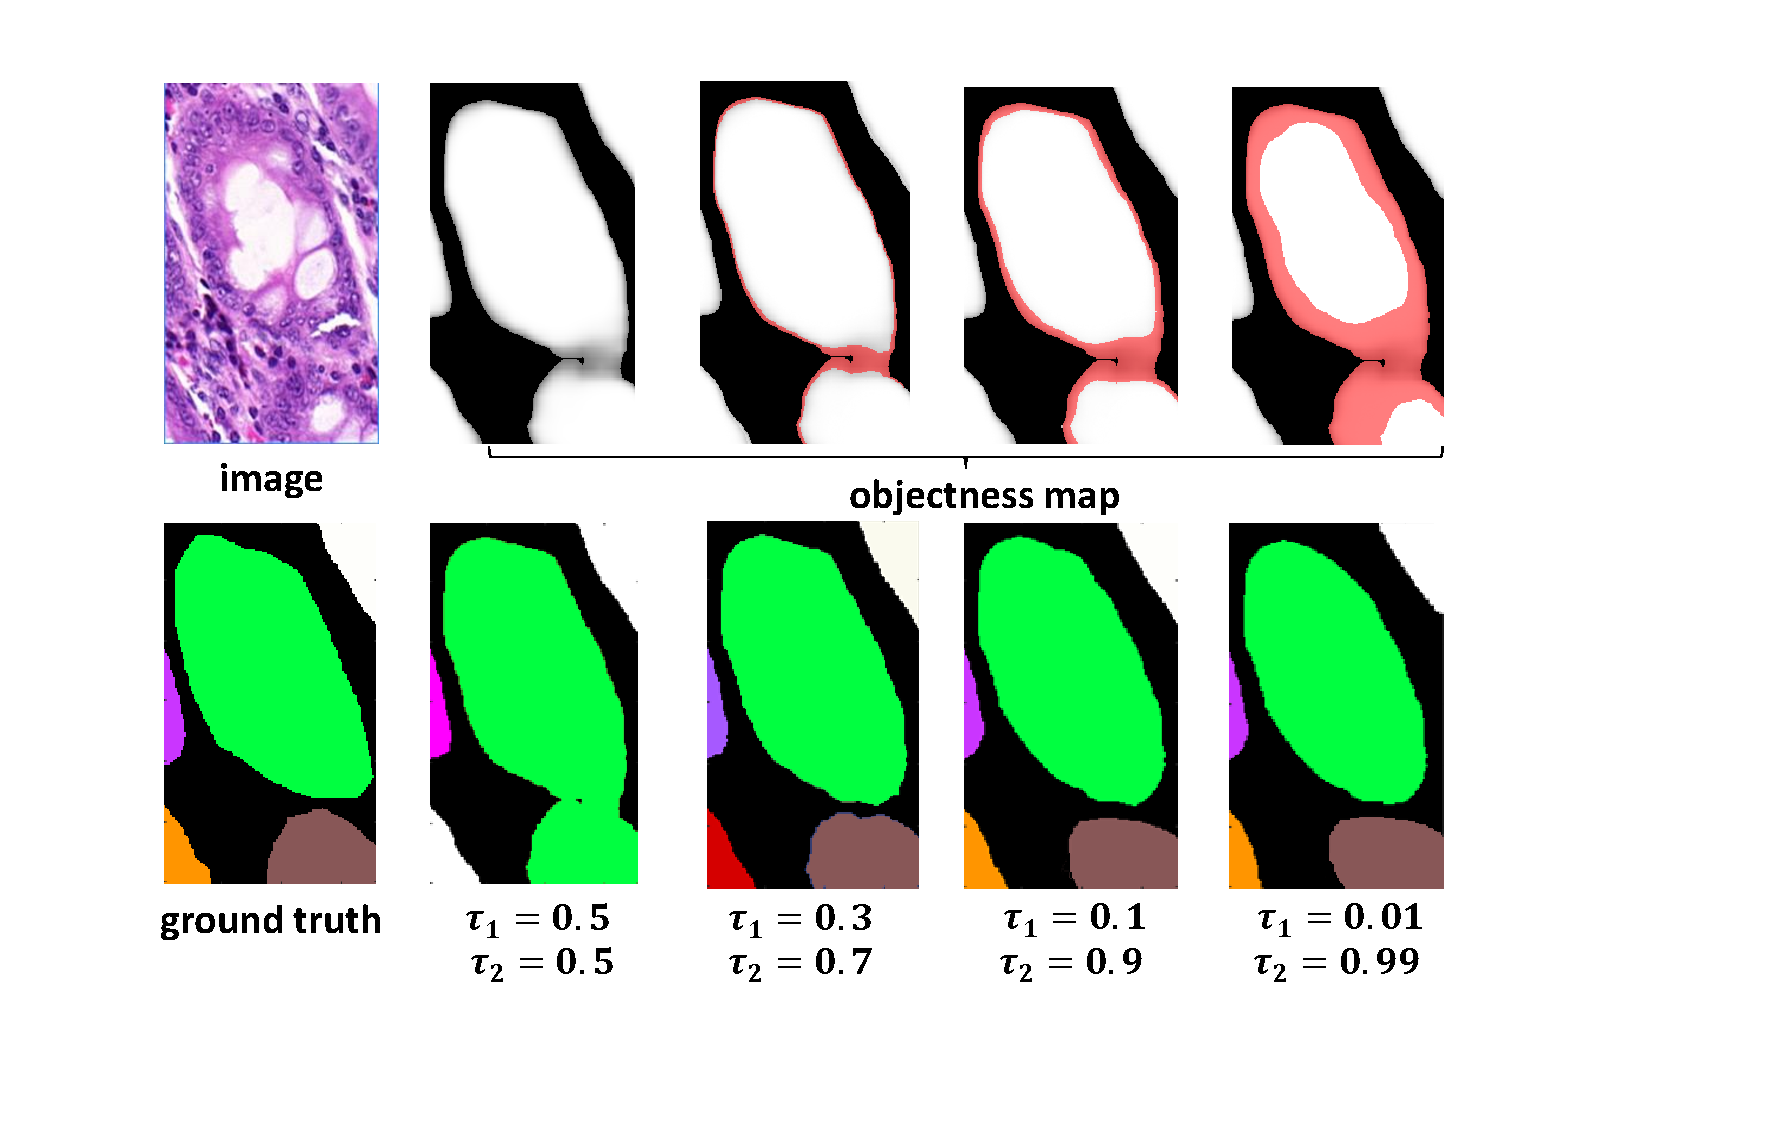
\includegraphics[width=3.4in]{figures/FigFusion.pdf}
   %\includegraphics[width=0.8\linewidth]{egfigure.eps}
    \end{center}
    \caption{Diagram of effects of varying $[\tau_1,\tau_2]$ to final segmentation (better seen in color).}
    \label{FigFusion}
\end{figure}
Especially, the range of $[\tau_1,\tau_2]$ controls the degree of regularity to the shape of segmented objects.
Figure~\ref{FigFusion} displays the changing process of objects shape with varying $[\tau_1,\tau_2]$.
It can be observed that, when the range of $[\tau_1,\tau_2]$ increases, the shape constraint on segmented objects becomes stronger.
And a small range of $[\tau_1,\tau_2]$ can retain the good generalization of model to irregular shape, while a larger range of $[\tau_1,\tau_2]$ performs better on separating objects apart and optimizing the shape of objects in terms of prior shape knowledge.
Therefore, the optimal $\tau_1, \tau_2$ should be determined by experiments so that both advantages of regularity and variety can be retained.
Furthermore any shape constraints can be easily incorporated by changing the definition in Eq.~\ref{EqPara}, if only the shape can be formulated by parameters.

